\documentclass[11pt,a4paper]{article}

\input{setup/project}
\input{setup/preamble}
\input{setup/weekly}

\renewcommand{\reportdate}{29 October 2026}

\begin{document}

\weeklytitle{9}

\section{Week 9: 26--30 October 2026}

\sectionprogress

\subsection*{Medis centerlines matched to the visual analysis}
All 600 trees were linked
through the study ID. As expected, almost all had plaque at baseline: 541 progressed and
58 were stable or regressed (Table~\ref{tab:medis}, Figure~\ref{fig:progression}). The
trees cannot be used for my main analysis of whether geometry predict plaque onset. Instead I tried to predict plaque progression of a segment.  

\begin{table}[h]
  \centering
  \small
  \caption{Outcome of the 600 patients with a Medis tree, by plaque status at baseline (rows) and
           at follow-up (columns). Plaque-free means $\mathrm{SIS} = 0$ and $\mathrm{SSS} = 0$.
           Worse means new plaque for a plaque-free patient, and a higher stenosis grade in at
           least one segment for a patient with plaque. Counts from 1 to 4 are shown as $<5$.}
  \label{tab:medis}

  \begin{tabular}{@{}lccc@{}}
    \toprule
    & \multicolumn{2}{c}{At FU, 10 years later} & \\
    \cmidrule(lr){2-3}
    At BL & Had segments progress & Stable / regressed & Total \\
    \midrule
    Plaque-free & $<5$ new plaque           & 0 never plaque                  & $<5$ \\[2pt]
    Plaque      & 541 progressed (90\,\%)   & 58 stayed or regressed (10\,\%) & 599 \\
    \midrule
    Total       &                           &                                 & 600 \\
    \bottomrule
  \end{tabular}
\end{table}

\begin{figure}[h]
  \centering
  \includegraphics[width=1\textwidth]{week_figure/progression_pie.png}
  \caption{Outcome at follow-up of the 600 patients with a Medis tree.}
  \label{fig:progression}
\end{figure}

\subsection{Centerlines cut into proximal, mid and distal}
The segments in the visual analysis are not necessarily cut the same way as the Medis centerline
labels, but I still chose to use them, and I will cut up the centerlines Kit delivers for all
patients the same way, because the plaque outcome is graded per segment and I want to utilise the detailed data set to its fullest. I believe the geometry to be a better predictor when it is measured locally, so if there are some error, it is worth if and should still give a better picture than averaging the whole artery. 

Each artery is followed from where it starts (the LM bifurcation for the LAD and LCx, the
ostium for the RCA) to its last point. Medis has given every centerline point the name of its
segment (pLAD, mLAD, \ldots), so I put the boundaries where the name changes. An unnamed stretch
between two names is split in the middle. Two cases need another rule:
\begin{itemize}
  \item \textbf{LCx.} Medis uses one name for everything after pCx, so I cut mid from distal at
        the first side branch that is named OM2 or is at least 15~mm long (not OM1), or halfway
        if there is no such branch.
  \item \textbf{No segment names.} Here I use anatomical landmarks.
        \emph{LAD:} proximal ends at the first diagonal, mid halfway to the end.
        \emph{LCx:} proximal ends at OM1, mid at OM2 (or halfway).
        \emph{RCA:} distal ends at the crux (where the PDA leaves), mid at the acute margin (the
        point farthest from the straight line from ostium to crux), proximal halfway to the
        acute margin.
        If a landmark branch has no name, the first side branch of at least 15~mm takes its
        place. If there is none, I use a fixed share of the artery: the first quarter for pLAD,
        the first third for pCX, and the end of the artery for the crux.
\end{itemize}

\textbf{Possible sanity check.} As I understand it, there was some strong connection between Medis contour and if the reader found plaque in that segment.  If the split is right, a segment graded moderate or worse in the visual analysis should
have a Medis contour lying inside that segment of my split artery. 

\subsection{Progression prediction model}
With the arteries split, I fitted a separate
logistic model for each of the nine segments of the LAD, LCx and RCA, predicting whether the visual grade of
that segment was higher at follow-up than at baseline. Each segment has two models: a base
model with log SCORE2, log follow-up time and the baseline grade of the segment, and the
same model with geometry added: the mean turning angle (T5) of the segment, plus the LM
bifurcation angle for pLAD and pCX. For segment $s$ of person $i$, the model sums the
variables, each multiplied by a weight, into a score
\begin{equation}
  \begin{split}
  \eta_i = {} & \beta_0 + \beta_1 \log(\mathrm{SCORE2}_i) + \beta_2 \log(\text{follow-up}_i)
                + \beta_3 \,\mathbf{1}[\text{BL grade} = \text{minimal}] \\
              & + \beta_4 \,\mathbf{1}[\text{BL grade} = \text{mild}]
                + \beta_5 \,\mathbf{1}[\text{BL grade} \geq \text{moderate}]
                + \gamma\, \mathrm{T5}_{is},
  \end{split}
  \label{eq:logit}
\end{equation}
where $\gamma = 0$ in the base model and the pLAD and pCX models also add a term for the LM
bifurcation angle. The score can take any value, and the logistic function turns it into a
probability of progression between 0 and 1:
\begin{equation}
  P(\text{segment } s \text{ of person } i \text{ progresses}) = \frac{1}{1 + e^{-\eta_i}}.
  \label{eq:logistic}
\end{equation}
The weights are those that fit the training data best (maximum likelihood with a small ridge
penalty), and $e^{\gamma}$ is the odds ratio per SD of T5. People were split into five outer folds that serve as
test sets, and four inner folds inside each training set choose the ridge penalty and the
cut-off. All models share the same folds, so no person is in both training and test data.
The AUCs are from the test folds (Figure~\ref{fig:segauc}, Table~\ref{tab:segauc}).

The base model separates progressing from stable segments moderately,
with AUCs from 0.55 in mCX to 0.70 in pRCA. Adding geometry changes the AUC by at most
0.02 in eight of the nine segments, and every 95\,\% interval but one includes zero. The
exception is mRCA, where geometry lowers the AUC slightly ($-0.016$). The largest gain is in
dCX ($+0.044$), but with only 38 progressed segments the interval is wide and includes
zero. Nine segments were tested, so one $p < 0.05$ is expected by chance alone.

In these patients, who almost all had plaque at baseline, segment curvature and the LM
bifurcation angle add no discrimination beyond the risk factors and the baseline grade. The
result has two limits. It concerns progression of existing disease, not new plaque in the
plaque-free cohort, which is the thesis question. It tests only two of the planned geometric
features: taper and the LM$\to$LAD and LM$\to$LCx diameter ratios need the lumen size along every
vessel, and Medis has lumen contours only for diseased segments. Whether geometry carries
signal therefore remains open until all features can be measured on the plaque-free cohort.

\begin{figure}[h]
  \centering
  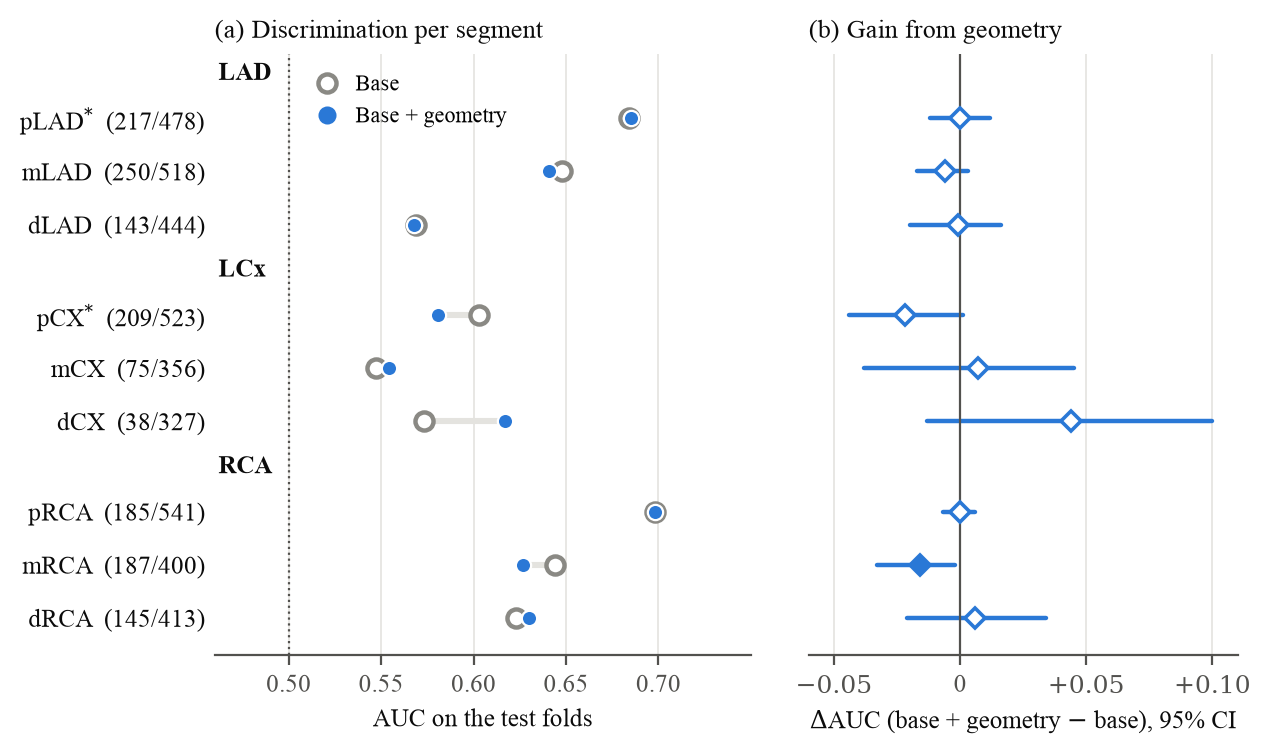
\includegraphics[width=1\textwidth]{week_figure/segment_auc.png}
  \caption{Segment progression in the Medis trees, base model vs base + geometry, one model per
           segment. (a) AUC on the test folds of the nested, person-split cross-validation; the
           dotted line is chance. In brackets: progressed / segments. $^{*}$ The LM bifurcation
           angle is included together with T5. (b) Change in AUC from adding geometry, with
           95\,\% bootstrap intervals; a filled marker means the interval excludes zero.}
  \label{fig:segauc}
\end{figure}

\begin{table}[h]
  \centering
  \small
  \setlength{\tabcolsep}{4pt}
  \caption{AUC per segment on the test folds. Base: log SCORE2, log follow-up time and baseline
           grade. Geometry: mean T5 of the segment; $^{*}$ also the LM bifurcation angle.
           $\Delta$AUC with 95\,\% bootstrap interval; $p$ from DeLong's test for paired AUCs.}
  \label{tab:segauc}

  \begin{tabular}{@{}llrccrr@{}}
    \toprule
    Artery & Segment & Progressed / $n$ & AUC base & AUC + geom. & $\Delta$AUC (95\,\% CI) & $p$ \\
    \midrule
    LAD & pLAD$^{*}$ & 217 / 478 & 0.684 & 0.685 & $+0.000$ ($-0.012$ to $+0.012$) & 0.98 \\
& mLAD & 250 / 518 & 0.648 & 0.641 & $-0.006$ ($-0.017$ to $+0.003$) & 0.25 \\
& dLAD & 143 / 444 & 0.569 & 0.568 & $-0.001$ ($-0.020$ to $+0.016$) & 0.91 \\[2pt]
    LCx & pCX$^{*}$ & 209 / 523 & 0.603 & 0.581 & $-0.022$ ($-0.044$ to $+0.001$) & 0.052 \\
& mCX  &  75 / 356 & 0.547 & 0.554 & $+0.007$ ($-0.038$ to $+0.045$) & 0.74 \\
& dCX  &  38 / 327 & 0.573 & 0.617 & $+0.044$ ($-0.013$ to $+0.100$) & 0.10 \\[2pt]
    RCA & pRCA & 185 / 541 & 0.698 & 0.698 & $-0.000$ ($-0.007$ to $+0.006$) & 0.96 \\
& mRCA & 187 / 400 & 0.644 & 0.627 & $-0.016$ ($-0.033$ to $-0.002$) & 0.034 \\
& dRCA & 145 / 413 & 0.623 & 0.630 & $+0.006$ ($-0.021$ to $+0.034$) & 0.65 \\
    \bottomrule
  \end{tabular}
\end{table}

\end{document}
